\begin{frame}
\begin{figure}[h!]
\centering
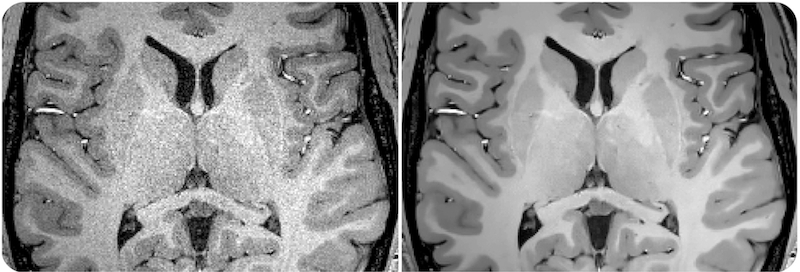
\includegraphics[width=0.9\textwidth]{./Images/denoise.jpg}
\end{figure}
\pause
\begin{figure}[h!]
\centering
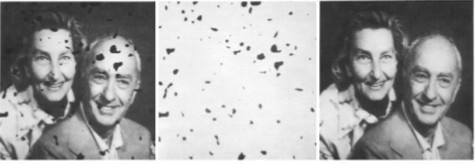
\includegraphics[width=0.9\textwidth]{./Images/inpaint.jpg}
\end{figure}
\end{frame}


\begin{frame}
\begin{figure}[h!]
\centering
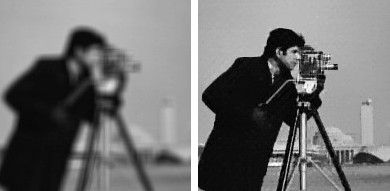
\includegraphics[width=0.7\textwidth]{./Images/deblurr.jpg}
\end{figure}
\pause
\begin{figure}[h!]
\centering
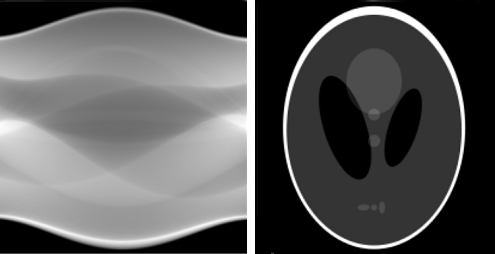
\includegraphics[width=0.7\textwidth]{./Images/CT.png}
\end{figure}
\end{frame}

\begin{frame}{Inverse problems in Imaging}
\begin{block}{\textbf{Goal}}
Recover parameters characterizing a system under investigation from measurements (e.g.\ recover image from data).
\end{block}
\pause
\bigskip

\begin{block}{Mathematical formulation}
Recover $f_{\text{true}}\in X$ from data
$$
g = \mathcal{T}(f_{\text{true}})+\delta g
$$
where $g\in Y$,$\mathcal{T}:X\longrightarrow Y$ and $\delta g\in Y$.
\end{block}

\pause
\bigskip

\begin{itemize}
\item \textbf{Classical solution:} 
Minimization of the miss-fit against data:
$$
\min_{f\in X}\mathcal{L}(\mathcal{T}(f),g)
$$
$\mathcal{L}:Y\times Y\longrightarrow \mathbb{R}$ is a transformation of the negative data log-likelihood ($-\log P(f|g)$), e.g. $\mathcal{L}(f)=||\mathcal{T}(f)-g||_2^2$.
\end{itemize}
\end{frame}

\begin{frame}{Ill-posedness and regularization}


\begin{block}{Hadamard well-posedness}
 Existence and uniqueness of solution for all data and continuous dependence of solution on the data.
\end{block}

\begin{block}{}
Ill-posed problems tend to produce overfitting when minimizing the data miss-fit, but they are the most common in applications (CT, EEG, MRI,...).
\end{block}

\bigskip
\pause
\begin{itemize}
\item \textbf{Regularization:} Set of methods to avoid overfitting by slightly modify the original problem to increase its regularity.

\bigskip
\pause
\item \textbf{Variational regularization:} Uses a functional $\mathcal{S}:X\longrightarrow \mathbb{R}$ (e.g. $||\cdot||_1$) to encode a priori information about $f_{\text{true}}$, obtaining:
$$
\min_{f\in X}\left[\mathcal{L}(\mathcal{T}(f),g)+\lambda \mathcal{S}(f)\right]\quad \text{for a fixed $\lambda\geq 0$}
$$

\end{itemize}
\end{frame}



\begin{frame}{Image denoising}
\begin{block}{\textbf{Goal}}
 Recover an image $f\in X$ from noisy data:
$$
g = f+\delta g
$$
where $\delta g$ is Gaussian white noise, with sd. $\sigma$.
\end{block}

\pause
\bigskip
\begin{itemize}
\item The risk of an estimator $\tilde{f}$ is given by the MSE:
$$
\mathbb{E}||f-\tilde{f}||_2^2
$$
$\mathbb{E}$ is the expectation with respect of the probability distribution of $\delta g$.
\pause
\bigskip
\item The worst behaviour of the estimator is the supremum
$$
\sup_{f\in X} \mathbb{E}||f-\tilde{f}||_2^2
$$
the \textit{Minimax} MSE will be
$$
\inf_{\tilde{f}}\sup_{f\in X}\mathbb{E}||f-\tilde{f}||^2_2
$$

\end{itemize}
\end{frame}

\begin{frame}{Minimax MSE}

\begin{block}{Frame}
A frame for a Hilbert space $X$ is a collection $\Psi=\{\psi_i\}_{i\in\mathcal{I}}\subset X$ satisfying
$$
A ||f||_2\leq ||\{\langle f,\psi_i\rangle\}_{i\in\mathcal{I}}||_{\ell^2(\mathcal{I})}\leq B||f||_2  \quad \forall f\in X
$$
for some $0<A\leq B<\infty$.
\end{block}

\
\pause

\begin{theorem}[(Labate et al., 2012)]
"If an image is sparse within a frame $\{\psi_i\}_{i\in \mathcal{I}}$, one can obtain a \textit{Minimax} MSE estimator by thresholding the coefficients in the expansion of the noisy data:
$$
g = \sum_{i\in\mathcal{I}}\langle g,\psi_i\rangle\psi_i \quad "
$$
\end{theorem}
\end{frame}

\begin{frame}{Image inpainting}

\begin{block}{\textbf{Goal}}
 Recover an image $f\in X$ from known data:
$$
g = P_K(f)
$$
where $P_K$ is and orthogonal projection onto the known subspace $X_K\triangleleft X$.
\end{block}

\pause
\bigskip

\begin{block}{\textbf{Sparse Regularization/CS approach (Genzel, Kutyniok):}}
 " If a signal (image) is sparse within a frame $\Psi$, it can be recovered from highly underdetermined, non-adaptive linear measurements by $\ell^1$-regularization (Davenport et al., 2012), i.e.
$$
\min_{\tilde{f}\in X}||\{\langle\tilde{f},\psi_i\rangle\}_{i\in\mathcal{I}}||_{\ell^1(\mathcal{I})} \quad \text{s.t. }P_K(\tilde{f})=g=P_K(f) \quad "
$$

\end{block}

\end{frame}

\begin{frame}

\begin{theorem}[Genzel, Kutyniok; 2014]
Let $\delta>0$ and $\Lambda\subset \mathcal{I}$ be a $\mathbf{\delta}$-\textbf{cluster} for $f$ with respect to a frame $\Psi$ (i.e.\ $||\mathbbm{1}_{\Lambda^c}T_{\Psi}f||_{\ell^1}\leq \delta$). If $\mu_c(\Lambda, P_M\Psi)<1/2$ and $f^*$ is the minimizer of the problem, then
$$
||\{\langle f^*-f,\psi_i\rangle\}_{i\in\mathcal{I}}||_{\ell^1(\mathcal{I})}\leq \frac{2\delta}{1-\mu_c(\Lambda,P_M\Psi)}
$$

\end{theorem}

\medskip

\begin{block}{Cluster coherence}
$$
\mu_c(\Lambda,P_M\Psi) :=\max_{j\in\mathcal{I}} \sum_{i\in \Lambda} |\langle P_M\psi_i,P_M\psi_j\rangle|
$$
\end{block}

\pause
\medskip
\begin{itemize}

\item \textbf{Conclusion:} One can use sparsifying frames on images to perform denoising and inpainting. The quality depends on the level of sparsity. 

\item \textbf{Problem:} Pick a good frame for the image space.
\end{itemize}
\end{frame} 

\begin{frame}{Image space: Cartoon-like functions}
\begin{definition}
Let $f:\mathbb{R}^2\longrightarrow\mathbb{C}$, $f\in\mathcal{E}^2(\mathbb{R}^2)$ if $f= f_0+\chi_B f_1$, with $B\subset [0,1]^2$, $\partial B\in C^2$ and with bounded curvature. Moreover, $f_i\in C^2(\mathbb{R}^2)$ with $||f_i||_{C^2}\leq 1$ and $\text{supp} f_i\subset [0,1]^2$ for $i=0,1$. 
\end{definition}
\pause
\begin{figure}[h!]
\centering
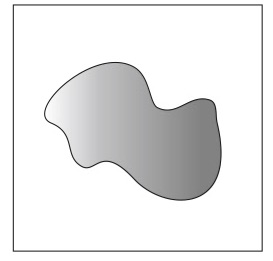
\includegraphics[width=0.4\textwidth]{./Images/cartoon-like.jpg}
\end{figure}
\end{frame}

\begin{frame}{Examples of frames for images}
\begin{itemize}
\item Gabor frames (Gabor, 1946).

\bigskip
\item Wavelet frames (Morlet et al., 1984).

\bigskip
\item Curvelet frames (Cand\`es et al., 1999).

\bigskip

\item Shearlet frames (Kutyniok et al., 2005).
\end{itemize}

\begin{figure}[h!]
\centering
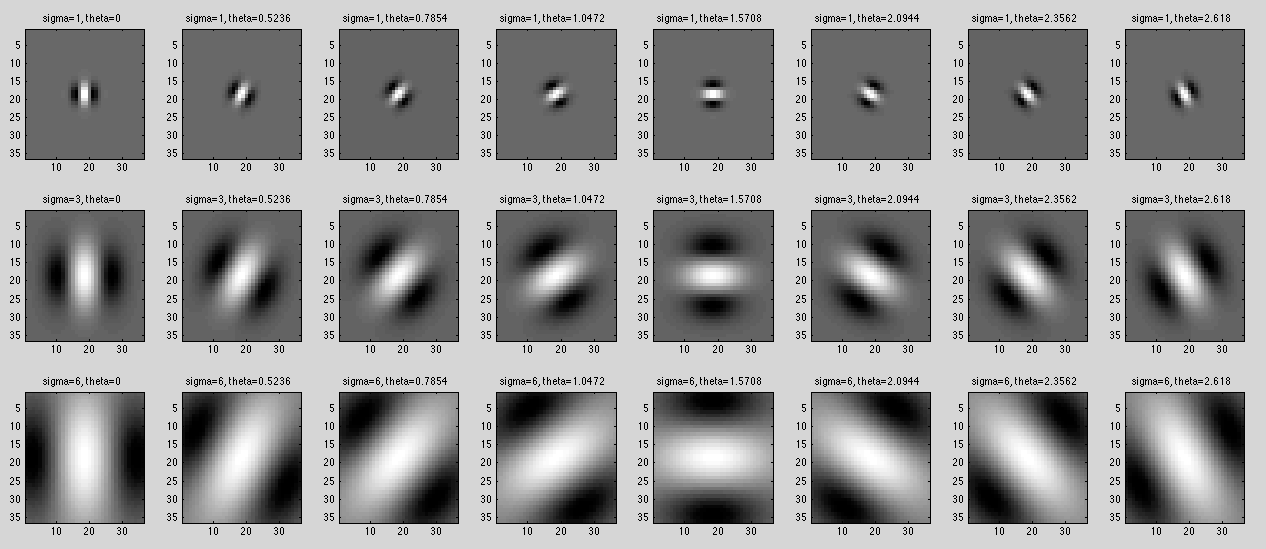
\includegraphics[width=0.8\textwidth, height=0.5\textheight]{./Images/STFTWave.png}
\end{figure}
\end{frame}


\begin{frame}{Optimal approximation error for images}
\begin{block}{Best N-term approx.\ error (Donoho, 2001)}
Let $\{\psi_{\lambda}\}_{\lambda\in\Lambda}\subset L^2(\mathbb{R}^2)$ a frame. The optimal best N-Term approximation error for any $f\in\mathcal{E}^2(\mathbb{R}^2)$ is
$$
\sigma_N(f,\{\psi_{\lambda}\}_{\lambda\in\Lambda})=O(N^{-1})
$$
\end{block}
\pause
\begin{block}{Error of 2D-wavelets}
$$
\sigma_N(f,\{\psi_{\lambda}\}_{\Lambda})\sim N^{-1/2}
$$
\end{block}
\pause
\end{frame}


\begin{frame}{Shearlet Transform (Kutyniok, Guo, Labate, 2005)}
\begin{block}{Classical Shearlet Transform}
$$
\langle f,\psi_{j,k,m}\rangle =\int_{\mathbb{R}^2}f(x)\overline{\psi_{j,k,m}(x)}dx
$$

where
$$
\mathcal{SH}(\psi)=\{\psi_{j,k,m}(x)=2^{3j/4}\psi (S_kA_jx-m):(j,k)\in\mathbb{Z}^2,m\in\mathbb{Z}^2\}
$$
\end{block}

\begin{figure}[h!]
\centering
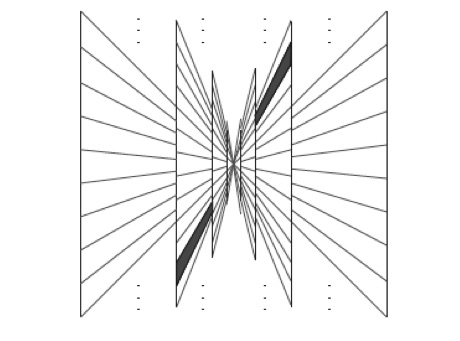
\includegraphics[width=0.4\textwidth]{./Images/tiling_nocone.jpg}
\end{figure}
\end{frame}

\begin{frame}{Cone-adapted shearlet transform and optimal sparsity}
$$
\mathcal{SH}(\phi,\psi,\tilde{\psi},c):=\mathcal{P}_{\mathcal{R}}\Phi(\phi,c1)\cup\mathcal{P}_{\mathcal{C}_1}\Psi(\psi,c)\cup\mathcal{P}_{\mathcal{C}_2}\tilde{\Psi}(\tilde{\psi,c})
$$

\begin{figure}[h!]
\centering
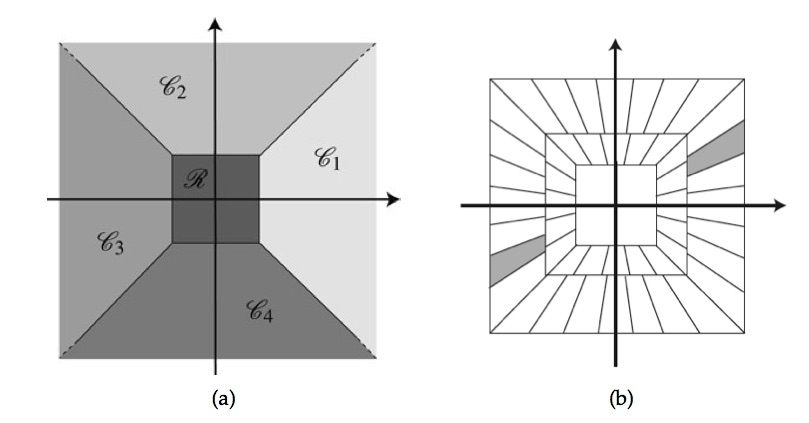
\includegraphics[width=0.6\textwidth]{./Images/tiling_cone}
\end{figure}

\pause
\begin{block}{\textbf{Cone shearlets sparsity} (Band limited case: Lim, Labate; 2006), (Compactly supported case: Kutyniok, Lim, 2011)}
Best $N$-term approximation error
$$
\sigma_N(f,\{\psi_{j,k,m}\}_{j,k,m})\sim N^{-1}(\log(N))^{3/2}
$$
\end{block}
\end{frame}


\begin{frame}{Current software}
\begin{itemize}
\item{Matlab}
\begin{itemize}
	\item FFST- Fast Finite Shearlet Transform (H\"auser, Steidl,TU Keiserslautern)\\ \url{http://www.mathematik.uni-kl.de/imagepro/software/ffst/}
	\item 2D/3D Shearlet Toolbox (D. Labate, University of Houston)\\ \url{https://www.math.uh.edu/~dlabate/software.html}
	\item \textbf{Shearlab3D} (G. Kutyniok, W.-Q.Lim, R. Reisenhofer, TU Berlin)\\\url{http://www.shearlab.org/}
\end{itemize}

\item{Python}
\begin{itemize}
	\item pyShearLab (Stefan Loock, U G\"ottingen) \\ \url{http://na.math.uni-goettingen.de/pyshearlab/}
\end{itemize}

\item{\textbf{Julia}}
\begin{itemize}
\item \textbf{Shearlab.jl} (H. Andrade, TU Berlin) \\ \url{https://github.com/arsenal9971/Shearlab.jl}
\end{itemize}

\pause

\item \textbf{Lets code!}
\end{itemize}
\end{frame}

\begin{frame}{Thanks!}
\begin{center}
\Large{Questions?}
\end{center}
\begin{figure}[h!]
\centering
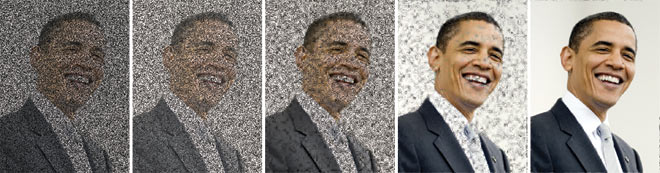
\includegraphics[width=1\textwidth]{./Images/obama_compressed.jpg}
\end{figure}
\end{frame}

